\section{Реализация}
Предложенный алгоритм был реализован в рамках исследовательского проекта YaccConstructor. В данной главе описывается архитектура предложенного решения: основные модули и их взаимодействие. Кроме того, рассматриваются особенности практической реализации.

\subsection{Архитектура предложенного решения}
На основе предложенного алгоритма разработан новый модуль инструмента YaccConstructor, который является генератором в терминах, принятых в этом проекте. Это показано на рис.~\ref{Arch}, где изображена архитектура инструмента YaccConstructor и цветом выделен реализованный модуль.

\begin{figure}[h]
 \centering
 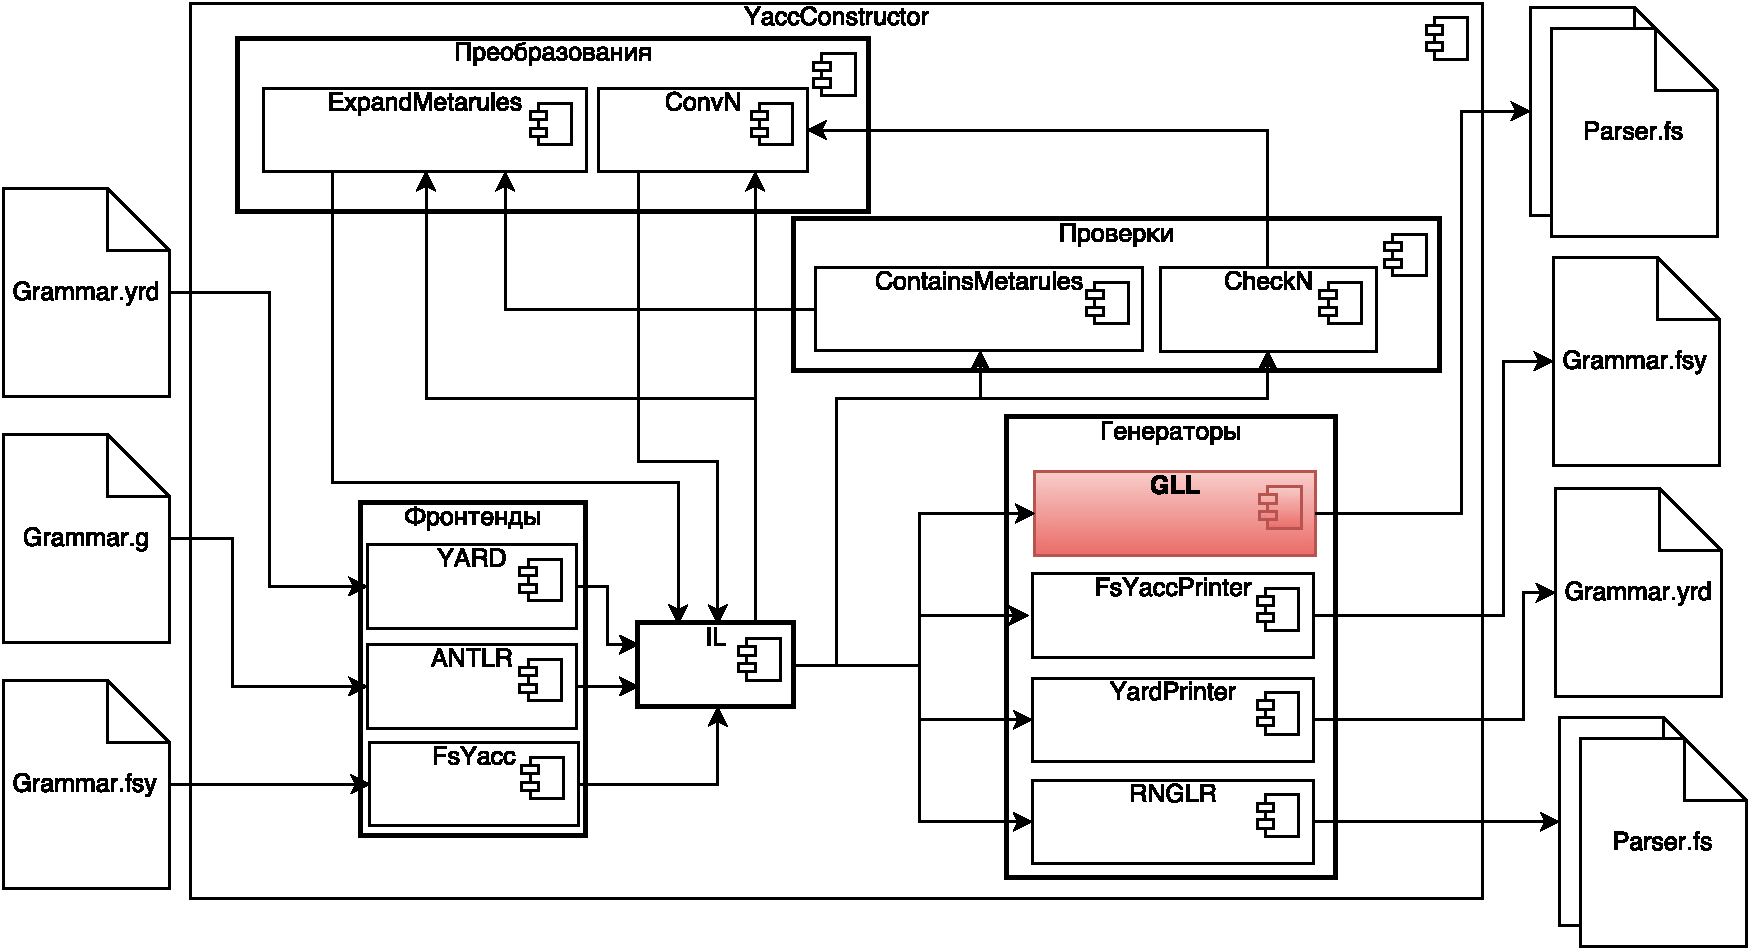
\includegraphics[width=\textwidth]{Ragozina/pics/Arch.pdf}
 \caption{Архитектура инструмента YaccConstructor (рисунок взят из работы~\cite{GrigorievPhd})}
 \label{Arch}
\end{figure}

Внутреннее устройство этого модуля показано на рис.~\ref{Arch2}. Основными компонентами являются генератор, который по грамматике строит управляющие таблицы и дополнительные структуры данных, компонента с описанием SPPF и функциями работы с ним, два интерпретатора управляющих таблиц, различающиеся тем, что один из них строит лес разбора, а другой нет. Интерпретаторы разделены в силу того, что структуры для хранения элементов дерева тесно связаны с другими структурами, используемыми при анализе, например, стеком, а отказ от построения леса был вызван необходимостью получить алгоритм, расходующий меньше памяти. По этой причине реализовано два набора структур данных, каждая из которых оптимальна при решении соответствующей задачи.

На вход генератор принимает внутреннее представление в формате IL, которое строится по грамматике и может быть получено с помощью соответствующего фронтенда. Так как в язык описания грамматики позволяет использовать конструкции, которые не обрабатываются генератором (например, метапрвила), то необходимо применить соответствующие преобразования, что достигается заданием специальных параметров при запуске инструмента. Результатом работы генератора является файл с исходным кодом, в котором описаны управляющие таблицы и вспомогательная информация, которая в дальнейшем используется интерпретатором. 

Интерпретатор написан вручную и содержит в себе основную логику алгоритма. Он подключается в виде отдельной сборки к целевому приложению и позволяет на основе сгенерированнх данных выполнять анализ входа.

Пользователь при создании приложения, использующего модуль, добавляет в свой проект сгенерированный файл, ссылку на интерпретатор и файл, содержащий лексический анализатор (полученный с помощью другого модуля YC, который не описывается в данной работе) и вызывает соответствующую функцию для синтаксического анализа. Результатом работы такой функции является либо SPPF, либо набор координат во входном графе, позволяющих определить положение в нём участка, порождающего строку, принимаемую соответствующей грамматикой.

\begin{figure}
 \centering
 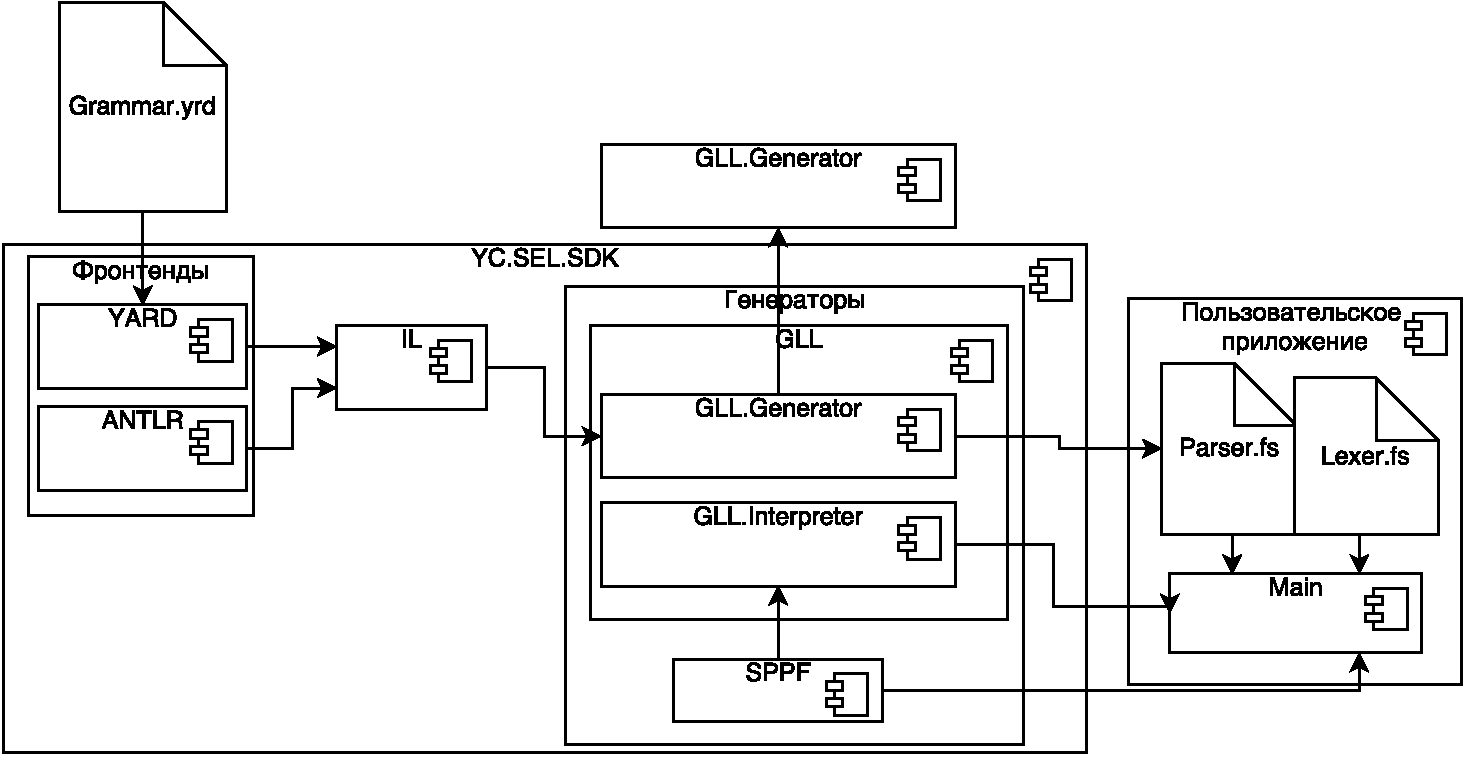
\includegraphics[width=\textwidth]{Ragozina/pics/GLL_Proc.pdf}
 \caption{Принцип работы реализованного модуля (рисунок взят и модифицирован из работы~\cite{GrigorievPhd})}
 \label{Arch2}
\end{figure}

\subsection{Особенности используемых структур данных}
Алгоритм реализован в рамках проекта YaccConstructor на языке программирования F\#. Исходный код свободно доступен в репозитории \url{https://github.com/YaccConstructor/YaccConstructor}, автор вёл разработку под учётной записью {\it AnastasiyaRagozina}.

Заявленная производительность алгоритма --- в худшем случае куб по памяти и времени --- обоснована теоретически~\cite{Johnstone201564}. На практике же, для достижения высокой производительности алгоритма, написанного с использованием языков высокого уровня, необходимо приложить некоторые усилия. Рассуждениям на данную тему и описанию эффективных структур данных посвящена работа~\cite{Johnstone2011}. При реализации описанного алгоритма подобные проблемы так же возникли: высокий расход памяти и медленные структуры данных. Основной проблемой было хранение леса разбора и поиск уже существующих узлов. Хранение узлов в многомерных массивах, как было предложено в ~\cite{Johnstone2011}, накладывало значительные ограничения на длину входа. Кроме того, хранение в каждом узле дерева нескольких чисел (имени нетерминала и координаты начала и конца подцепочки, соответствующей данному поддереву) делало его громоздким. В результате, для того, чтобы уменьшить расход памяти при хранении SPPF было использовано сжатие хранимых в узлах координат в одно число. Это позволило вместо хранения двух чисел хранить одно, которое можно было использовать в качестве ключа при поиске уже созданных поддеревьев. Аналогичное сжатие использовалось для хранения слотов. Для хранения терминальных узлов в алгоритме было предложено использовать динамически изменяемый массив,  размер которого сравним с размером входных данных, что приводит к выделению большого количества лишней памяти при использовании стандартного типа \verb|ResizeArray<_>| при больших размерах входа. Для решения этой проблемы использовалась модификация динамически изменяемого массива, в которой память выделяется блоками константного размера. Данная структура данных была реализована в рамках работы над RNGLR-алгоритмом. В рамках данной работы она была выделена в библиотеку структур данных \texttt{FSharpx.Collections}, поддерживаемую FSharp-сообществом~\cite{FsharpX}. Подобные задачи являются интересными с инженерной точки зрения и часто возникают на практике.

Важной задачей так же является представление метагеномной сборки и её обработка, так как, в отличие от графа, являющегося аппроксимацией встроенных языков, граф, представляющего метагеномную сборку, как правило, существенно большего размера. Для того, чтобы уменьшить размер самого графа, на рёбрах хранится не по одному токену, а цепочки токенов. Это приводит к тому, что теперь в качестве координаты начала и конца подстроки используется не два числа, а четыре --- номера рёбер и позиция на них. По аналогии, эти числа сжимались. Для того, чтобы эффективно использовать такие индексы была создана структура данных, доступ к элементам которой как у массива, но по сжатому числу. 

При обработке графа метагеномной сборки были использованы следующие знания о его структуре и особенностях решаемой задачи. В графе есть рёбра, на которых лежат подстроки длины большей, чем длина искомой подстроки. Это означает, что такие рёбра можно удалить из графа и обработать отдельно, как линейные данные. При этом граф распадается на набор связанных компонент, что позволяет обрабатывать части входного графа полностью независимо. Это, в свою очередь, существенно упрощает параллельную обработку данных: возникает классическая параллельность по данным, когда к большому количеству независимых данных нужно применить одну и ту же функцию обработки. 

Однако, несмотря на то, что параллельность по данным может быть реализована очевидным образом, использование нескольких потоков в рамках одного многоядерного процессора не даёт ожидаемого прироста производительности, что наглядно продемонстрировано на рис.~\ref{StackExp}.

\begin{figure}
 \centering
 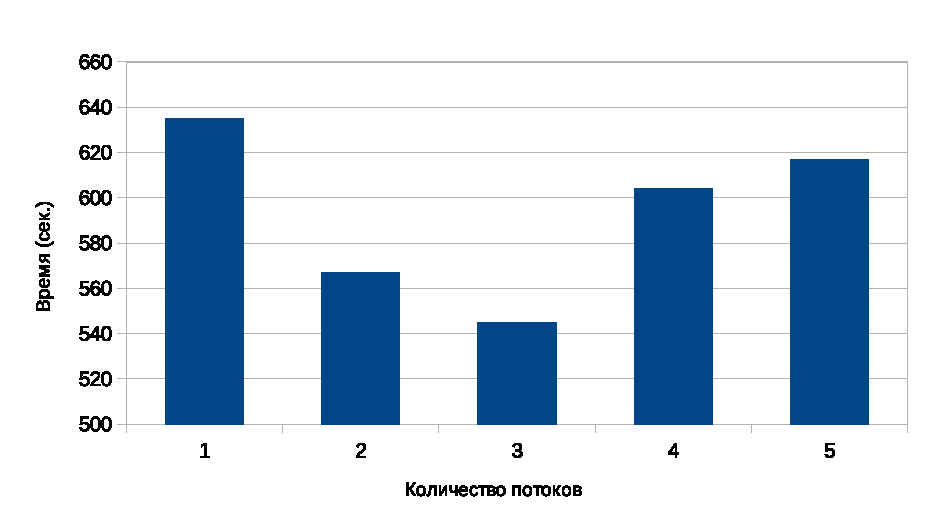
\includegraphics[width=\textwidth]{Ragozina/pics/Stack.pdf}
 \caption{Сравнение производительности предложенного решения при запуске на нескольких потоках }
 \label{StackExp}
\end{figure} 

Замеры, результаты которых представлены на рис.~\ref{StackExp} и рис.~\ref{StackExp2} проводились на машине со следующей конфигурацией:
\begin{itemize}
\item OS Name	Microsoft Windows 10 Pro
\item System Type x64-based PC
\item Processor	Intel(R) Core(TM) i7-4790 CPU 3.60GHz, 3601 Mhz, 4 Core(s), 4 Logical Processor(s)
\item Installed Physical Memory (RAM)	32.0 GB
\end{itemize}

Из рис.~\ref{StackExp} видно, что максимальная производительность наблюдается при использовании двух потоков. Однако прирост производительности по сравнению с использованием одного потока составляет всего 6.4\%, что значительно меньше теоретически возможного.

Такое поведение системы связано с тем, что при обработке одного графа происходит активное обращение к вспомогательным структурам данных большого объёма. При этом обращения, в силу особенностей алгоритма, плохо локализованы. В связи с чем, при попытке обработать несколько графов одновременно на одном процессоре, учащаются промахи кэшей. Частично решить эту проблему удалось заменив очередь дескрипторов на стек, это сделало обращения к данным более локализованными и позволило улучшить производительность решения. 

Результаты измерений после замены очереди на стек представлены на рис.~\ref{StackExp2}. Максимальная производительность достигается при использовании трёх потоков и прирост производительность составляет 14.2\%. На рис.~\ref{StackExp2} представлено сравнение производительности до и после модификации.



\begin{figure}
 \centering
 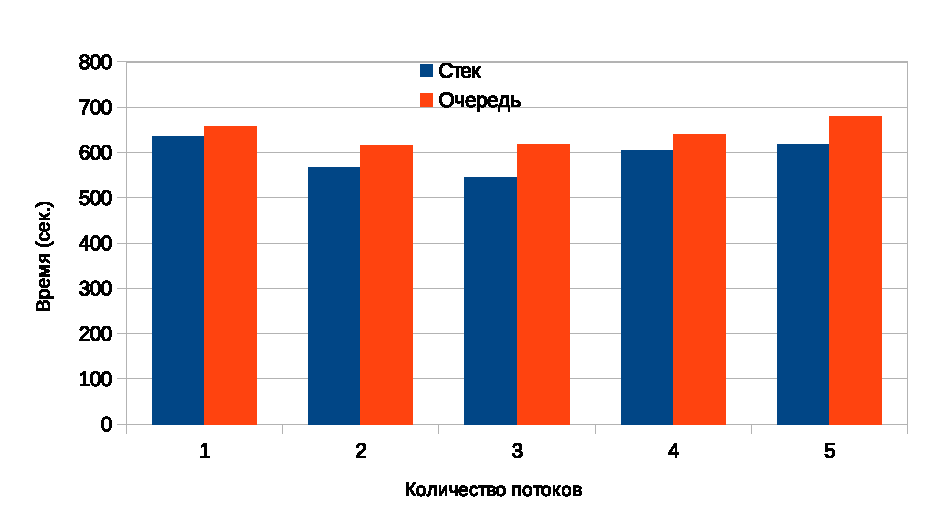
\includegraphics[width=\textwidth]{Ragozina/pics/StackVSQueue.pdf}
 \caption{Сравнение производительности предложенного решения замене стека на очередь для хранения дескрипторов }
 \label{StackExp2}
\end{figure}

Для того, чтобы избавиться от проблем с кэшами при многопоточной обработке, можно использовать многопроцессорные системы, такие как вычислительные кластеры. При этом, как показали проведённые ранее эксперименты, имеет смысл запускать не более двух потоков на одном процессоре. Так как время обработки одного подграфа занимает время порядка нескольких секунд, то затраты на передачу по сети не должны заметно уменьшать выигрыш, получаемый за счёт параллельной обработки при достаточном количестве графов для обработки на одном узле.  

Для реализации вычислений в кластере была выбрана технология MBrace, которое позволяет, с одной стороны, управлять кластером в облаке Microsoft.Azure с помощью скриптов на F\#. Предоставляется полный набор функций, позволяющий сконфигурировать кластер ``с нуля'', а затем управлять им (например, изменять количество машин). С другой стороны, MBrace позволяет прозрачно использовать кластер в коде на F\#. Это достигается благодаря предоставлению набора высокоуровневых функций и окружения \texttt{cloud}, благодаря которому код, предназначенный для выполнения в кластере можно задать следующим образом.

\begin{listing}
    \begin{pyglist}[language=ocaml,numbers=left,numbersep=5pt]
    
let parallelTask = 
    [ for i in 1 .. 10 -> 
          cloud { return sprintf "i'm work item %d" i } ]
    |> Cloud.Parallel
    |> cluster.CreateProcess

\end{pyglist}
\caption{Код для запуска предложенного решения в кластере}
\label{lst:mbraceExample}
\end{listing}

В скобках \verb|cloud { }| может находиться произвольный код на F\#. Все необходимые для выполнения этого кода в кластере дополнительные действия и коммуникации (передача данных, подготовка и передача бинарных файлов) осуществляется автоматически и не требует участия разработчика. Таким образом, в предположении, что функция обработки графа \texttt{processGraph}  реализована и всё, что необходимо для реализации обработки массива графов о кластере, это ``завернуть'' её вызов в окружение \texttt{cloud} следующим образом.

\begin{listing}
    \begin{pyglist}[language=ocaml,numbers=left,numbersep=5pt]
    
let parallelGraphProcessing graphs = 
    [ for g in graphs -> cloud { return processGraph g } ]
    |> Cloud.Parallel
    |> cluster.CreateProcess

\end{pyglist}
\caption{Код для запуска предложенного решения в кластере с параметризацией входных данных}
\label{lst:mbraceExample}
\end{listing}
